% !TEX root = cha-implementation.tex
\documentclass[../../main.tex]{subfiles}

\begin{document}

\section{Class Layout and Placement}

The placement process converts the structural relationships between classes into positions on the grid. The implementation follows the steps described in \secref{sec:layout_via_MDS}: computing pairwise distances, obtaining a two dimensional embedding using metric Multidimensional Scaling (mMDS), mapping the resulting coordinates to grid positions, and placing the classes while respecting the defined constraints.

\subsection{Distance Matrix and MDS}
First, an $n \times n$ distance matrix is created, where $n$ is the number of classes. The diagonal is initialized to zero, while all other entries are initialized to infinity. Direct relationships are then used to fill the distances between connected classes. The distance of a relationship is computed as the reciprocal of its weight (\equref{eq:class-distance}), so stronger relationships result in smaller distances.

After the direct distances have been added, the Floyd-Warshall algorithm~\citebibliography{Floy1962a} (presented in \algref{alg:floyd-warshall}) is used to compute the shortest distance between every pair of classes. This enrich the distance matrix with indirect relationships.

\begin{algorithm}
\caption{Floyd-Warshall}
\label{alg:floyd-warshall}
\begin{algorithmic}[1]
\STATE Initialize matrix $D$ with direct relationship distances
\FOR{$k = 1$ \TO $n$}
    \FOR{$i = 1$ \TO $n$}
        \FOR{$j = 1$ \TO $n$}
            \STATE $D[i,j] \gets \min(D[i,j], D[i,k] + D[k,j])$
        \ENDFOR
    \ENDFOR
\ENDFOR
\end{algorithmic}
\end{algorithm}

\figref{fig:distance-matrix} shows an example of the distance matrix before and after applying Floyd-Warshall. 

\begin{figure}[ht]
    \centering
    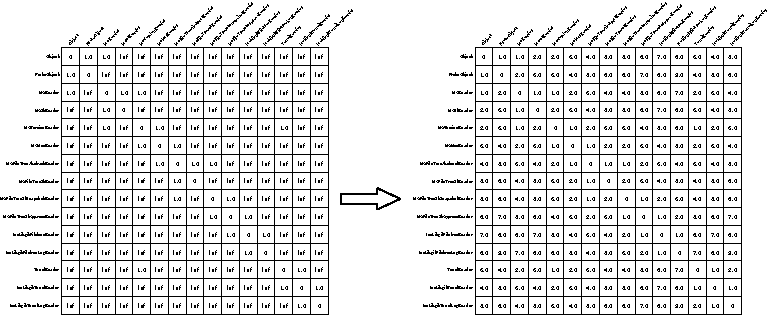
\includegraphics[width=\linewidth]{figures/implementation/distance_calculation}
    \caption{Distance matrix before and after Floyd-Warshall.}
    \label{fig:distance-matrix}
\end{figure}

Classes that remain disconnected after Floyd-Warshall are assigned a distance larger than the graph diameter. This keeps disconnected classes farther from the others in the layout calculated by mMDS.

Before running mMDS, a power transformation can be applied to the distances. Each distance $\delta_{ij}$ is transformed into $\delta_{ij}^{p}$, where $p$ is a configurable parameter. When $p > 1$, larger distances are emphasized compared to smaller ones. When $0 < p < 1$, smaller distances are emphasized compared to larger ones.

The resulting distance matrix is given to mMDS. The implementation uses the SMACOF iterative optimization proceess. It starts with random positions and updates them iteratively to reduce the difference between the target distances and the Euclidean distances between the classes. The process stops when the maximum number of iterations is reached or when the change in stress becomes smaller than the configured tolerance.

The result is a 2D position for each class. These positions are normalized to the range $[0,1]$ using a global minimum ($v_{\min}$) and maximum ($v_{\max}$), considering all values across both dimensions.

Each coordinate $v$ is normalized as follows:
\begin{equation}
    v_{\text{norm}} =
    \begin{cases}
        0.5 & \text{if } v_{\max} - v_{\min} = 0, \\
        \frac{v - v_{\min}}{v_{\max} - v_{\min}} & \text{otherwise.}
    \end{cases}
\end{equation}

If all classes collapse to the exact same position (\ie $v_{\max} - v_{\min} = 0$), all normalized coordinates are set to $0.5$ as a fallback.

\subsection{Mapping Positions to the Grid}

The normalized coordinates are scaled to the grid size. For each dimension, the normalized value in $[0,1]$ is multiplied by the current grid size $n$, and the result is rounded to the nearest integer.

This produces discrete integer coordinates for each class on the grid. Since mMDS can place classes at identical or very close positions, the normalization, scaling, and rounding process may map multiple classes to the same target position.

\subsection{Class Placement}

Classes are placed on the grid according to the positions computed by mMDS. Since a class can occupy multiple cells, its area is represented as a \texttt{WSFootprint}. The footprint contains the nodes occupied by the class, its top-left node, and its side length. A class is always represented by a square footprint.

For each class, the algorithm first tries to use its target position. A position is valid only if the footprint fits in the grid and the required distance from other classes is maintained. If the target position is not valid, the algorithm searches for candidates in expanding rings around the target position, starting from the first ring. For each ring, all valid positions are collected. If at least one valid position is found, the search stops and the best candidate among those positions is selected.

When multiple candidates are found in the same ring, the candidate with the smallest total Manhattan distance to already placed connected classes is selected. The Manhattan distance between two classes is computed from their border cells. If the class has no connected classes placed yet, one of the valid candidates is selected at random. If no valid position is found in a ring, the algorithm checks the next ring. If no valid position can be found, the placement fails, the grid is expanded, and the placement process  restarts.

After all classes have been placed, the nodes in each footprint are converted into class tiles.

\subsection{Path Exit Assignment}

Once a class has been placed, its border cells are used as entry and exit points for its paths. These exits are assigned before running WFC, as they provide the constraints needed to generate paths between classes. Without these, WFC would have no information about where paths should connect to the class footprints.

The exits assignment is performed in two steps. First, the algorithm computes a preference order for each path ID of each class. Second, it assigns each path ID to a specific border cell based on these preferences.

\paragraph{Directional Preference Calculation}

For each path ID in the system, the algorithm computes a target position as the centroid of all classes connected by that path ID. For this calculus, the position of a class is defined as the center of its footprint. If the footprint has an even side length, one of its four central cells is selected at random.

Then, for each path ID of each class, a vector $\mathbf{A}$ is computed from the center of the class to the target position of the path ID. This vector represents the ideal direction in which the path should leave the class.

The algorithm compares $\mathbf{A}$ with the four directions: up $(0,1)$, down $(0,-1)$, right $(1,0)$, and left $(-1,0)$, using cosine similarity:

\begin{equation}
    \mathrm{cosineSimilarity}(\mathbf{A},\mathbf{B}) = \frac{\mathbf{A}\cdot\mathbf{B}}{|\mathbf{A}||\mathbf{B}|}.
\end{equation}

Cosine similarity measures how well a direction matches the direction towards the target. Its value ranges from $-1$ to $1$. A value close to $1$ means that the two directions are aligned, a value close to $-1$ means that they point in opposite directions, and a value of $0$ means that they are orthogonal.

Since the algorithm uses costs that have to be minimized, cosine similarity is converted into a cost:

\begin{equation}
    \mathrm{cost}(\mathbf{A},\mathbf{B}) = 1-\mathrm{cosineSimilarity}(\mathbf{A},\mathbf{B}).
\end{equation}

Therefore:

\begin{itemize}
    \item $\mathrm{cost}=0$ represents a perfect alignment ($\mathrm{cosineSimilarity}=1$);
    \item $\mathrm{cost}=1$ represents an orthogonal direction ($\mathrm{cosineSimilarity}=0$);
    \item $\mathrm{cost}=2$ represents the worst direction ($\mathrm{cosineSimilarity}=-1$).
\end{itemize}

The four grid directions are then sorted by increasing cost. This produces an ordered list of preferred directions for each path ID of a class. The first direction is therefore the preferred one.

An example is provided in \figref{fig:cosine_similarity}. Since the source class has a $3 \times 3$ footprint, its center cell is used as the reference position. The target position (centroid) results in a vector $\mathbf{A} = (6,2)$ from the class center. Comparing this vector with the four grid directions gives the following costs: up $= 0.658$, left $= 1.949$, right $= 0.051$, and down $= 1.316$. The directions are therefore ordered as right, up, down, and left. % The right direction is the preferred direction for this path ID, making the right side of the top-right cell of the class footprint the most likely location for the path exit.

\begin{figure}[ht]
    \centering
    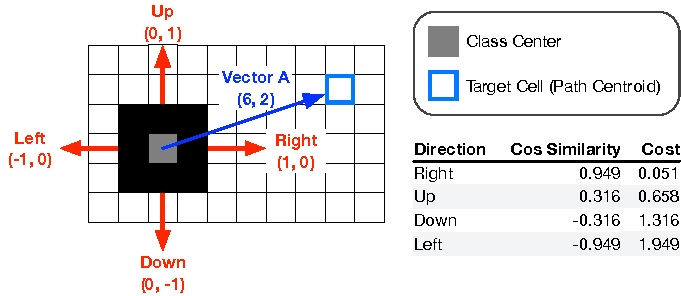
\includegraphics[width=0.92\linewidth]{figures/implementation/cosine_similarity}
    \caption{Example of preferred direction of a path ID calculation.}
    \label{fig:cosine_similarity}
\end{figure}

\paragraph{Border Cell Assignment}

After computing the preferred directions, each path is assigned to a specific border cell of the class footprint. Each path has an ordered list of preferred directions, from the most to the least preferred one. The assignment is performed as follows:

\begin{enumerate}

    \item Paths are first grouped by their primary preferred direction. Each group corresponds to one side of the class footprint, and paths in the same group compete for the cells available on that side.

    \item Within each group, paths are ordered by their primary direction cost. Paths with lower costs are assigned first. This gives priority to the paths that have a stronger preference for that side when there are more paths than available cells.

    \item For each path, its secondary direction is used to determine its position along the side. The path is assigned to the first available cell in the direction of its secondary preference. For example, if the primary direction is \textit{right} and the secondary direction is \textit{up}, the path is assigned to the highest available cell on the right side (\ie the cell with the minimum row index).

    \item If all cells on a side are already assigned, the remaining paths are moved to the group corresponding to their next preferred direction. When a path is moved to a new group, the direction of the side where it was originally placed becomes its secondary direction. More generally, the secondary direction is the first preferred direction that is different from the direction of the group. For example, if a path has the preference order \textit{up}, \textit{left}, \textit{down}, \textit{right}, but there is no available cell in the \textit{up} group, it is moved to the \textit{left} group. In this case, \textit{up} becomes its secondary direction and is used to choose its position on the left side.

    \item The process is repeated until all paths have been assigned.

\end{enumerate}

This approach keeps paths with similar directions close to each other and helps reduce crossings immediately after leaving the class. As the footprint size of each class is computed from its total number of connections, enough border cells are available to place all its paths.

\end{document}